\label{frame-sync}
The Frame synchronization is an enhancement proposal on top of the chunk model. Here, instead of using video chunks, each crowdworker receives the key-frames sequences from two videos that must be synchronized. This way, each worker has access to the full video at once, enhancing the possibilities of finding a synchronization point. However, as now the worker interacts with frames, if a pair of frames is identified as a possible synchronization point, its precision is reduced, making necessary a second step on the task: watch the videos based on the information provided by the two frames (each frame has a timestamp from when it which part of the video it was removed, making possible to calculate $\Delta$ such as in the chunk based one).

Figure~\ref{frames} shows the interface developed to this approach: on the top the user selects the probably aligned frames (or close ones) and plays the videos. If it is correct, he confirms the alignment, else he tries again or discard the synchronization. 

\begin{figure}[h]
	\centerline{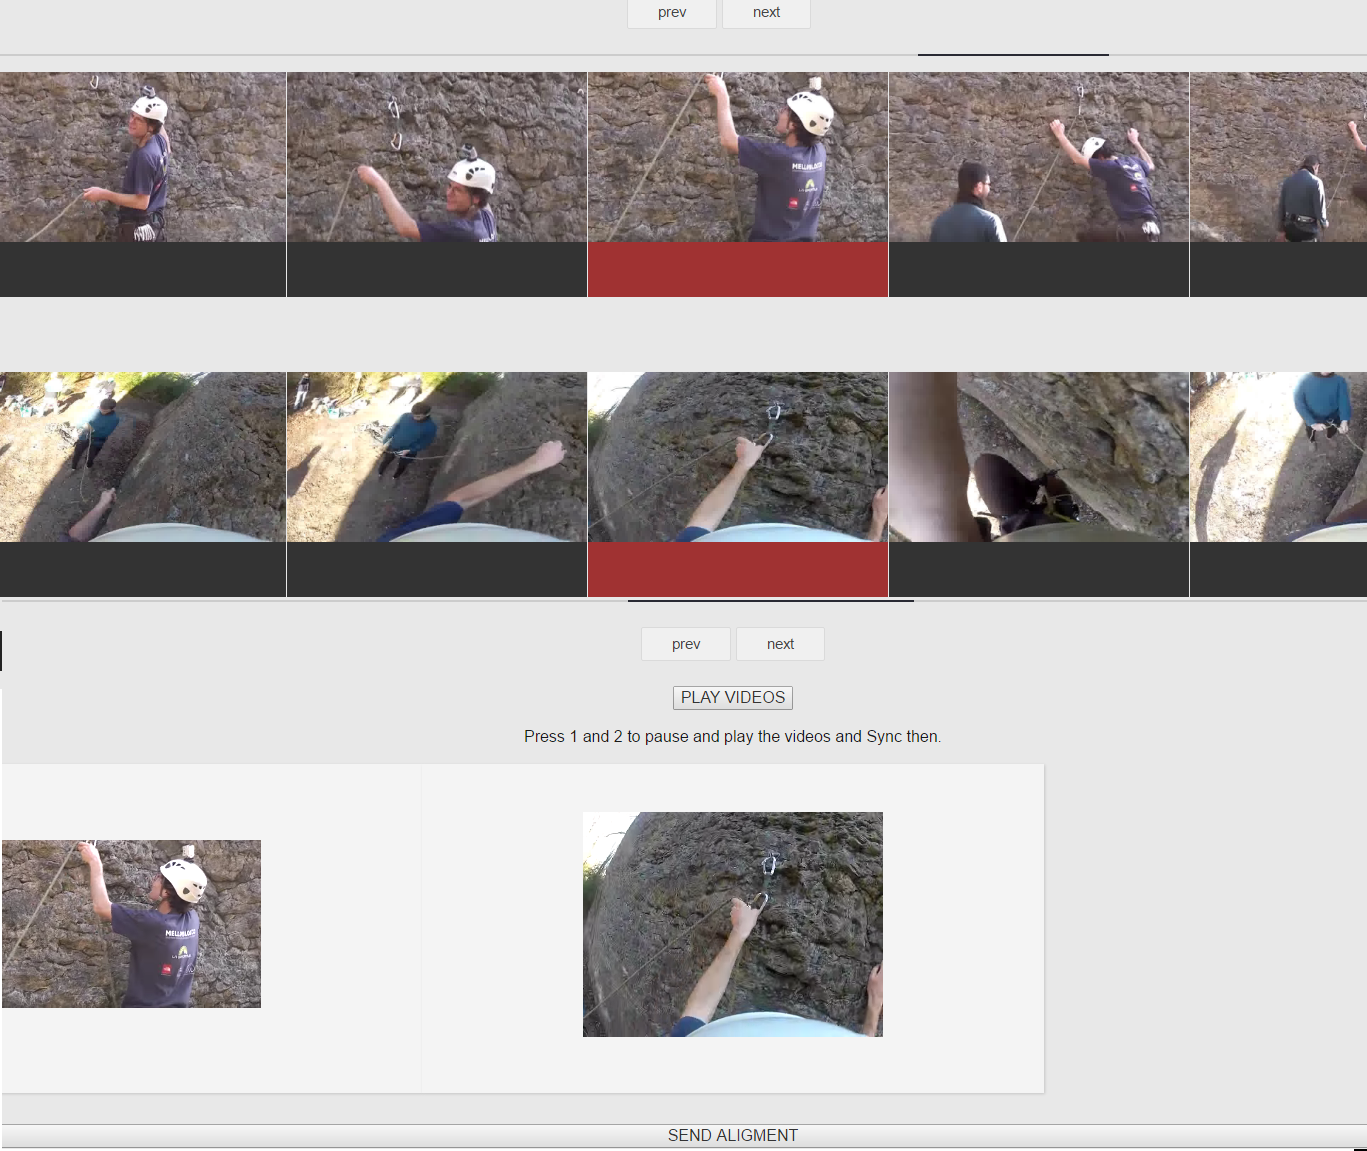
\includegraphics[scale=0.25] {figure/frames}}
	\caption{Frame Synchronization Method}
	\label{frames}
\end{figure}